% Goursat's subdivision: a triangle, its four midpoint triangles, and two further generations. Generated by a short script.
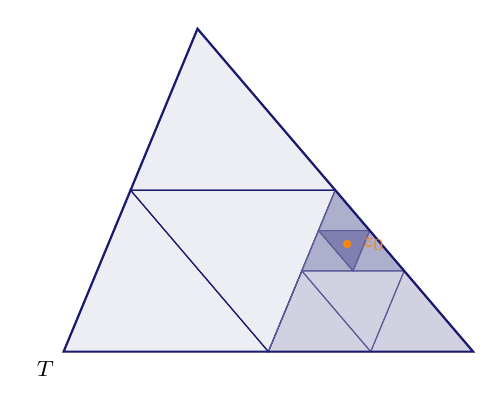
\begin{tikzpicture}[every node/.style={font=\footnotesize}]
\fill[MidnightBlue!8] (0.000,0.000)--(5.200,0.000)--(1.700,4.100)--cycle;
\fill[MidnightBlue!20] (2.600,0.000)--(5.200,0.000)--(3.450,2.050)--cycle;
\draw[MidnightBlue] (0.000,0.000)--(2.600,0.000)--(0.850,2.050)--cycle;
\draw[MidnightBlue] (2.600,0.000)--(5.200,0.000)--(3.450,2.050)--cycle;
\draw[MidnightBlue] (0.850,2.050)--(3.450,2.050)--(1.700,4.100)--cycle;
\draw[MidnightBlue] (2.600,0.000)--(3.450,2.050)--(0.850,2.050)--cycle;
\fill[MidnightBlue!35] (3.025,1.025)--(4.325,1.025)--(3.450,2.050)--cycle;
\draw[MidnightBlue!70] (2.600,0.000)--(3.900,0.000)--(3.025,1.025)--cycle;
\draw[MidnightBlue!70] (3.900,0.000)--(5.200,0.000)--(4.325,1.025)--cycle;
\draw[MidnightBlue!70] (3.025,1.025)--(4.325,1.025)--(3.450,2.050)--cycle;
\draw[MidnightBlue!70] (3.900,0.000)--(4.325,1.025)--(3.025,1.025)--cycle;
\fill[MidnightBlue!55] (3.675,1.025)--(3.888,1.537)--(3.238,1.537)--cycle;
\draw[MidnightBlue!70] (3.025,1.025)--(3.675,1.025)--(3.238,1.537)--cycle;
\draw[MidnightBlue!70] (3.675,1.025)--(4.325,1.025)--(3.888,1.537)--cycle;
\draw[MidnightBlue!70] (3.238,1.537)--(3.888,1.537)--(3.450,2.050)--cycle;
\draw[MidnightBlue!70] (3.675,1.025)--(3.888,1.537)--(3.238,1.537)--cycle;
\draw[MidnightBlue,thick] (0.000,0.000)--(5.200,0.000)--(1.700,4.100)--cycle;
\fill[BurntOrange] (3.600,1.367) circle (1.5pt) node[right=2pt,BurntOrange] {$z_0$};
\node[below left] at (0.000,0.000) {$T$};
\end{tikzpicture}
